\subsubsection{Coarse Grids}\label{subsubsection: Coarse Grids}

\textbf{\underline{Purpose}}. Simplifies the problem by \textbf{reducing the number of grid points}, capturing broad features, and addressing low-frequency errors. In other words, reduce the grids with fewer points and greater spacing between them compared to the fine grid.

\highspace
Before we go any further, we need to understand the \textbf{difference between Coarse and Fine Grid}. This can be done from an image point of view, for example, an image where we can see the simplification of details:
\begin{figure}[!htp]
    \centering
    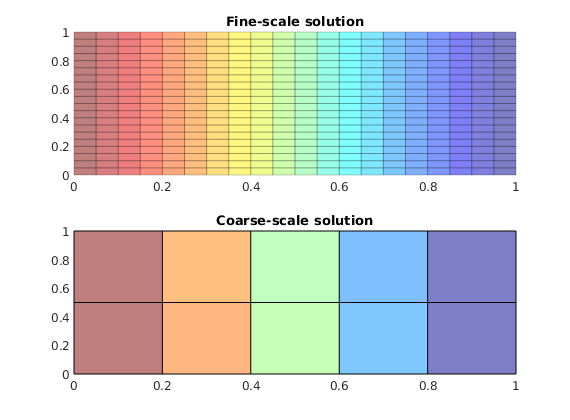
\includegraphics[width=\textwidth]{img/coarsegrid-1.png}
    \caption{Difference between Coarse and Fine Grid.}
\end{figure}

\noindent
But to understand frequency, we have to look at the problem from a one-dimensional point of view, looking at frequencies.
\begin{itemize}
    \item \textbf{Fine Grid} has a high resolution, then many closely spaced points.
    \begin{center}
        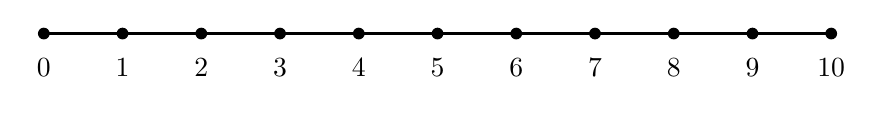
\begin{tikzpicture}
            \def\n{10}
            \foreach \i in {0,...,\n} {
                \node[circle, fill=black, inner sep=1.5pt] at (\i,0) {};
                \node[below] at (\i,-0.2) {\i};
                \ifnum\i>0
                    \draw[thick] (\i-1,0) -- (\i,0);
                \fi
            }
        \end{tikzpicture}
    \end{center}

    \item \textbf{Coarse Grid} has a lower resolution, then fewer points spaced farther apart.
    \begin{center}
        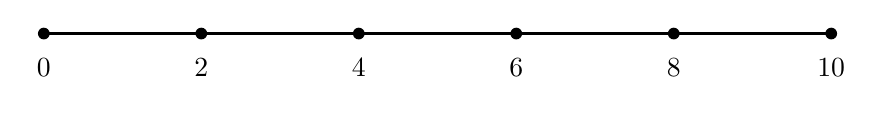
\begin{tikzpicture}
            \foreach \i/\label in {0/0, 1/2, 2/4, 3/6, 4/8, 5/10} {
                \node[circle, fill=black, inner sep=1.5pt] at (\i*2,0) {};
                \node[below] at (\i*2,-0.2) {\label};
                \ifnum\i>0
                    \draw[thick] (\i*2-2,0) -- (\i*2,0);
                \fi
            }
        \end{tikzpicture}
    \end{center}
\end{itemize}

\newpage

\noindent
As we \textbf{move from the fine grid to the coarse grid, the mode becomes more oscillatory because the same error pattern spans fewer points, increasing its apparent frequency}. The term \dquotes{mode} refers to the different error patterns or components in the solution. See the following illustration for a 100\% understanding.

\highspace
Consider a wave function on the fine grid $w_{j} = \sin\left(\dfrac{j \pi}{n+1} i \right)$ (where $j$ determines the frequency, $n$ is the number of points, and $i$ is the index of the grid point), its 1D representation, and the signal:
\begin{center}
    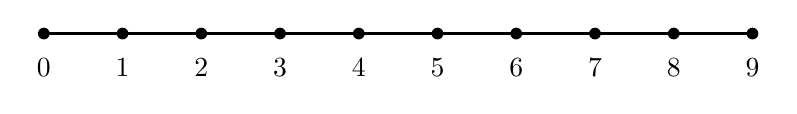
\begin{tikzpicture}
        \def\n{9}
        \foreach \i in {0,...,\n} {
            \node[circle, fill=black, inner sep=1.5pt] at (\i,0) {};
            \node[below] at (\i,-0.2) {\i};
            \ifnum\i>0
                \draw[thick] (\i-1,0) -- (\i,0);
            \fi
        }
    \end{tikzpicture}
\end{center}
\begin{center}
    \begin{tikzpicture}
        \draw[->] (-0.5,0) -- (11,0) node[right] {$i$};
        \draw[->] (0,-1.5) -- (0,1.5);
        \node at (-0.2, -0.3) {$0$};

        \draw[thick] plot[domain=0:9.9,samples=1000] (\x,{sin(deg(10*\x*pi/11))});
        
        \foreach \k in {0, 1.1, 2.2, 3.3, 4.4, 5.5, 6.6, 7.7, 8.8, 9.9} {
            \node[circle, fill=black, inner sep=1.5pt] at (\k,0) {};
        }

        \node at (10,2) {$w_{10} = \sin\left(\dfrac{10 \pi}{11} i \right)$};
        \node at (7,2) {$n = 10$};
        \node at (5,2) {$j = 10$};
    \end{tikzpicture}
\end{center}

\noindent
If we pass from the Fine Grid to Coarse Grid reducing the number of points, for example from 10 to 6, we obtain an increase of the oscillatory and also the same error pattern is repeated several times:
\begin{center}
    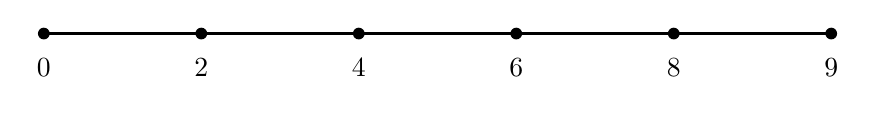
\begin{tikzpicture}
        \foreach \i/\label in {0/0, 1/2, 2/4, 3/6, 4/8, 5/9} {
            \node[circle, fill=black, inner sep=1.5pt] at (\i*2,0) {};
            \node[below] at (\i*2,-0.2) {\label};
            \ifnum\i>0
                \draw[thick] (\i*2-2,0) -- (\i*2,0);
            \fi
        }
    \end{tikzpicture}
\end{center}
\begin{center}
    \begin{tikzpicture}
        \draw[->] (-0.5,0) -- (11,0) node[right] {$i$};
        \draw[->] (0,-1.5) -- (0,1.5);
        \node at (-0.2, -0.3) {$0$};

        \draw[thick] plot[domain=0:9.9,samples=1000] (\x,{sin(deg(10*\x*pi/7))});

        \node at (10,2) {$w_{10} = \sin\left(\dfrac{10 \pi}{7} i \right)$};
        \node at (7,2) {$n = 6$};
        \node at (5,2) {$j = 10$};
    \end{tikzpicture}
\end{center}
\newpage
\begin{center}
    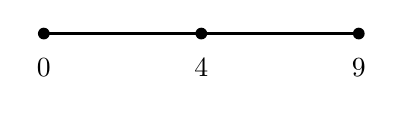
\begin{tikzpicture}
        \foreach \i/\label in {0/0, 1/4, 2/9} {
            \node[circle, fill=black, inner sep=1.5pt] at (\i*2,0) {};
            \node[below] at (\i*2,-0.2) {\label};
            \ifnum\i>0
                \draw[thick] (\i*2-2,0) -- (\i*2,0);
            \fi
        }
    \end{tikzpicture}
\end{center}
\begin{center}
    \begin{tikzpicture}
        \draw[->] (-0.5,0) -- (11,0) node[right] {$i$};
        \draw[->] (0,-1.5) -- (0,1.5);
        \node at (-0.2, -0.3) {$0$};

        \draw[thick] plot[domain=0:9.9,samples=1000] (\x,{sin(deg(10*\x*pi/4))});

        \node at (10,2) {$w_{10} = \sin\left(\dfrac{10 \pi}{4} i \right)$};
        \node at (7,2) {$n = 3$};
        \node at (5,2) {$j = 10$};
    \end{tikzpicture}
\end{center}

\noindent
Obviously, \textbf{smooth modes on a Fine Grid will look less smooth on a Coarse Grid}.